\documentclass{article}
\usepackage{tikz}
\usepackage{pgfplots}
\usepackage{amsmath}
\usetikzlibrary{3d,calc}

\begin{document}

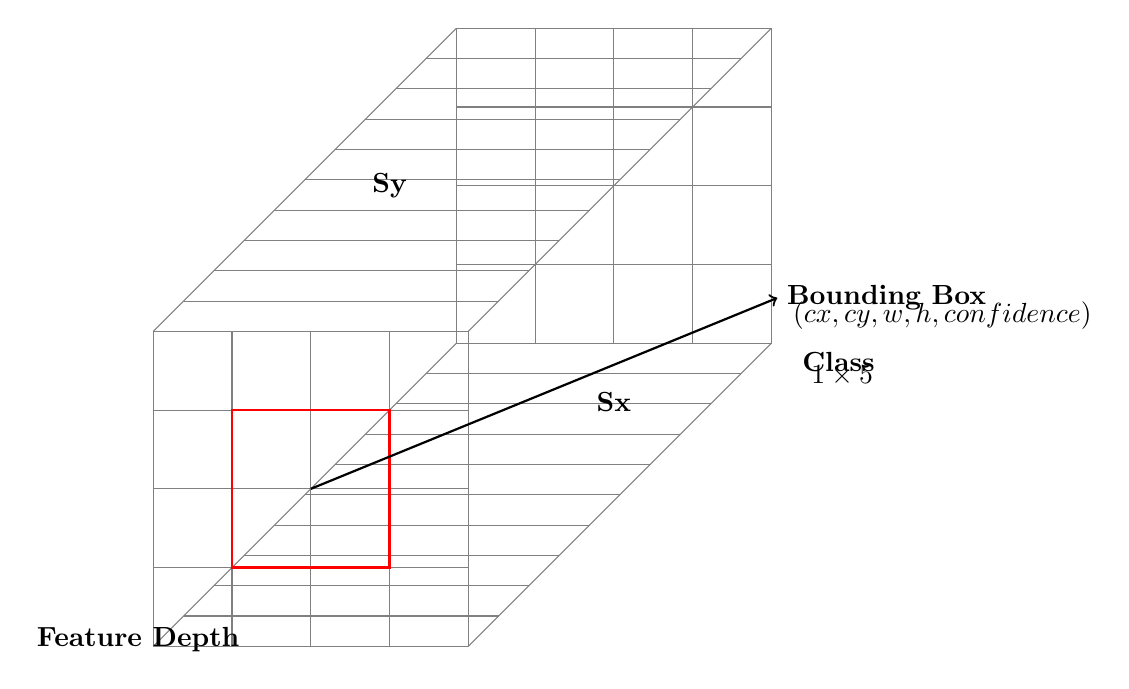
\begin{tikzpicture}

    % 立方体参数
    \def\Sx{4}    % 正面 x 方向网格数
    \def\Sy{4}    % 正面 y 方向网格数
    \def\Depth{10} % 深度(横向网格数)

    % 绘制 3D 立方体
    \draw[gray, thin] (0,0,0) -- ++(\Sx,0,0) -- ++(0,\Sy,0) -- ++(-\Sx,0,0) -- cycle;
    \draw[gray, thin] (0,0,\Depth) -- ++(\Sx,0,0) -- ++(0,\Sy,0) -- ++(-\Sx,0,0) -- cycle;
    \draw[gray, thin] (0,0,0) -- ++(0,0,\Depth);
    \draw[gray, thin] (\Sx,0,0) -- ++(0,0,\Depth);
    \draw[gray, thin] (0,\Sy,0) -- ++(0,0,\Depth);
    \draw[gray, thin] (\Sx,\Sy,0) -- ++(0,0,\Depth);

    % 画内部网格
    \foreach \x in {1,...,\Sx} {
        \draw[gray, thin] (\x,0,0) -- ++(0,\Sy,0);
        \draw[gray, thin] (\x,0,\Depth) -- ++(0,\Sy,0);
    }
    \foreach \y in {1,...,\Sy} {
        \draw[gray, thin] (0,\y,0) -- ++(\Sx,0,0);
        \draw[gray, thin] (0,\y,\Depth) -- ++(\Sx,0,0);
    }
    \foreach \z in {1,...,\Depth} {
        \draw[gray, thin] (0,0,\z) -- ++(\Sx,0,0);
        \draw[gray, thin] (0,\Sy,\z) -- ++(\Sx,0,0);
    }

    % 画 Bounding Box
    \draw[thick, red] (1,1,\Depth) -- (3,1,\Depth) -- (3,3,\Depth) -- (1,3,\Depth) -- cycle;
    
    % 连接 Bounding Box 说明
    \draw[->, thick] (2,2,\Depth) -- (6,2.5,5);
    
    % 标注 Bounding Box 参数
    \node[right] at (6,2.5,5) {\textbf{Bounding Box}};
    \node[right] at (6,2.2,4.8) {$(cx, cy, w, h, confidence)$};
    
    % 标注类别信息
    \node[right] at (6,1.5,4.5) {\textbf{Class}};
    \node[right] at (6,1.2,4.2) {$1 \times 5$};

    % 轴标签
    \node[below] at (\Sx/2, -0.5, 0) {\textbf{Sx}};
    \node[left] at (-0.5, \Sy/2, 0) {\textbf{Sy}};
    \node[above] at (0, 0, \Depth+0.5) {\textbf{Feature Depth}};

\end{tikzpicture}

\end{document}
